\documentclass[11pt]{articulo}
\usepackage{amsmath}
\usepackage{graphicx}

\baselineskip 25pt
\textwidth 15cm
\textheight 23cm
\topmargin -1.5cm
\oddsidemargin 1cm 
\evensidemargin 1cm 

\begin{document}

\title{\bf Laboratorio de F\'isica I\\
  Gu\'ia del experimento \emph{P\'endulo de Pohl}}
\author{
  {\bf J\'onatan Piedra}\\
  Universidad de Cantabria}
\maketitle


\section{Introducci\'on}

El objetivo de esta pr\'actica es estudiar experimentalmente mediante un p\'endulo de torsi\'on de Pohl el movimiento oscilatorio libre, amortiguado y forzado. Se determinar\'an las frecuencias caracter\'isticas de las oscilaciones libres, el decrecimiento exponencial de amplitud en las oscilaciones amortiguadas y la curva de resonancia de las oscilaciones forzadas.


\section{Fundamento te\'orico}

El p\'endulo de Pohl consta de un disco plano que gira respecto a un eje perpendicular al mismo. El disco est\'a conectado a un muelle espiral, de tal manera que cuando se separa el disco de su punto de equilibrio un \'angulo $\phi$ el muelle trata de devolverlo a su posici\'on de equilibrio, estableci\'endose as\'i un movimiento oscilatorio. Conectado al p\'endulo hay un freno electromagn\'etico que amortigua las oscilaciones, y un motor que act\'ua como forzamiento. De este modo el p\'endulo de Pohl permite un estudio de las oscilaciones libres, amortiguadas y forzadas.

\subsection{Oscilaciones libres}

Al desplazar el disco un cierto \'angulo $\phi$ respecto de su posici\'on de equilibrio y dejarlo libre, debido al muelle act\'ua sobre el disco un momento de reacci\'on proporcional a $\phi$. Si se considera despreciable la fuerza de rozamiento con el aire, y si no act\'ua ninguna fuerza de frenado, el p\'endulo sigue un movimiento arm\'onico $\phi (t) = \phi_0 \cos (\omega_0 t + \delta_0)$, donde $\omega_0$ es la frecuencia propia del p\'endulo.

\subsection{Oscilaciones amortiguadas}

Cuando se tiene en cuenta la p\'erdida de energ\'ia debida a fuerzas de rozamiento se obtiene una oscilaci\'on amortiguada. Para velocidades peque\~nas se puede considerar que el momento producido por la fuerza de amortiguamiento es proporcional a la velocidad angular. En esta situaci\'on cuando $\gamma < \omega_0$ (oscilaciones subamortiguadas) se obtiene
%
\begin{equation*}
\phi (t) = \phi_0 \exp(-\gamma t) \cos(\omega_A t + \delta_0),
\end{equation*}
%
donde $\gamma$ es el coeficiente de amortiguamiento y la frecuencia para el movimiento amortiguado es $\omega_A = \sqrt{\omega_0^2 - \gamma^2}$. En los tiempos $t_n$ en los que el coseno toma los valores $+1$ (m\'aximos) y $-1$ (m\'inimos) se obtiene $\left|\phi\left(t_n\right)\right| = \left|\phi_0\right|\exp\left(-\gamma t_n\right)$.

\subsection{Oscilaciones forzadas}

En las oscilaciones amortiguadas la amplitud, y por tanto la energ\'ia, decrece con el tiempo hasta que el p\'endulo se para. Para mantener las oscilaciones se utiliza un motor que proporciona un forzamiento peri\'odico de frecuencia $\Omega$. En el estado estacionario se obtiene el movimiento arm\'onico $\phi(t) = A \cos ( \Omega t + \delta)$. El valor de la amplitud $A$ viene dado~\cite{morin} por la expresi\'on
%
\begin{equation*}
A = \frac{F_0/m}{\sqrt{\left(\omega_0^2 - \Omega^2\right)^2 + 4 \gamma^2\Omega^2}}.
\end{equation*}
%
La amplitud de las oscilaciones alcanza el valor m\'aximo para la frecuencia de resonancia $\Omega_r = \sqrt{\omega_0^2 - 2\gamma^2}$.


\section{Dispositivo experimental}

Se dispone de un p\'endulo de torsi\'on de Pohl con un freno electromagn\'etico para amortiguar las oscilaciones. El funcionamiento de este freno est\'a basado en la generaci\'on de corrientes de Foucault sobre el disco de cobre debidas al campo magn\'etico que crea el electroim\'an colocado en la base del p\'endulo. El electroim\'an est\'a alimentado con corriente continua y la intensidad se mide con un amper\'imetro colocado en serie. {\bf ADVERTENCIA IMPORTANTE: el freno electromagn\'etico soporta una intensidad m\'axima de 1~A.} Para las oscilaciones forzadas se dispone de un motor el\'ectrico que permite aplicar al p\'endulo una fuerza peri\'odica de frecuencia variable $\Omega$, a trav\'es de una palanca que lo conecta al resorte. La frecuencia de las oscilaciones forzadas $\Omega$ puede modificarse con los dos botones de control grueso y fino situados en la parte superior del motor, el cual est\'a alimentado con corriente continua y el voltaje se mide mediante dos conexiones situadas en la parte inferior del motor. {\bf ADVERTENCIA IMPORTANTE: el motor soporta una intensidad m\'axima de 650~mA.} Para las medidas del per\'iodo y de la amplitud de las oscilaciones se dispone de un sensor de rotaci\'on conectado a un ordenador. El dispositivo experimental se puede observar en la Figura~\ref{pohl}. {\bf Se toma el valor de 0,01~s como incertidumbre en la posici\'on de cada m\'aximo (o m\'inimo).}
%
\begin{figure}[htb]
\begin{center}
\hspace*{0.0cm}
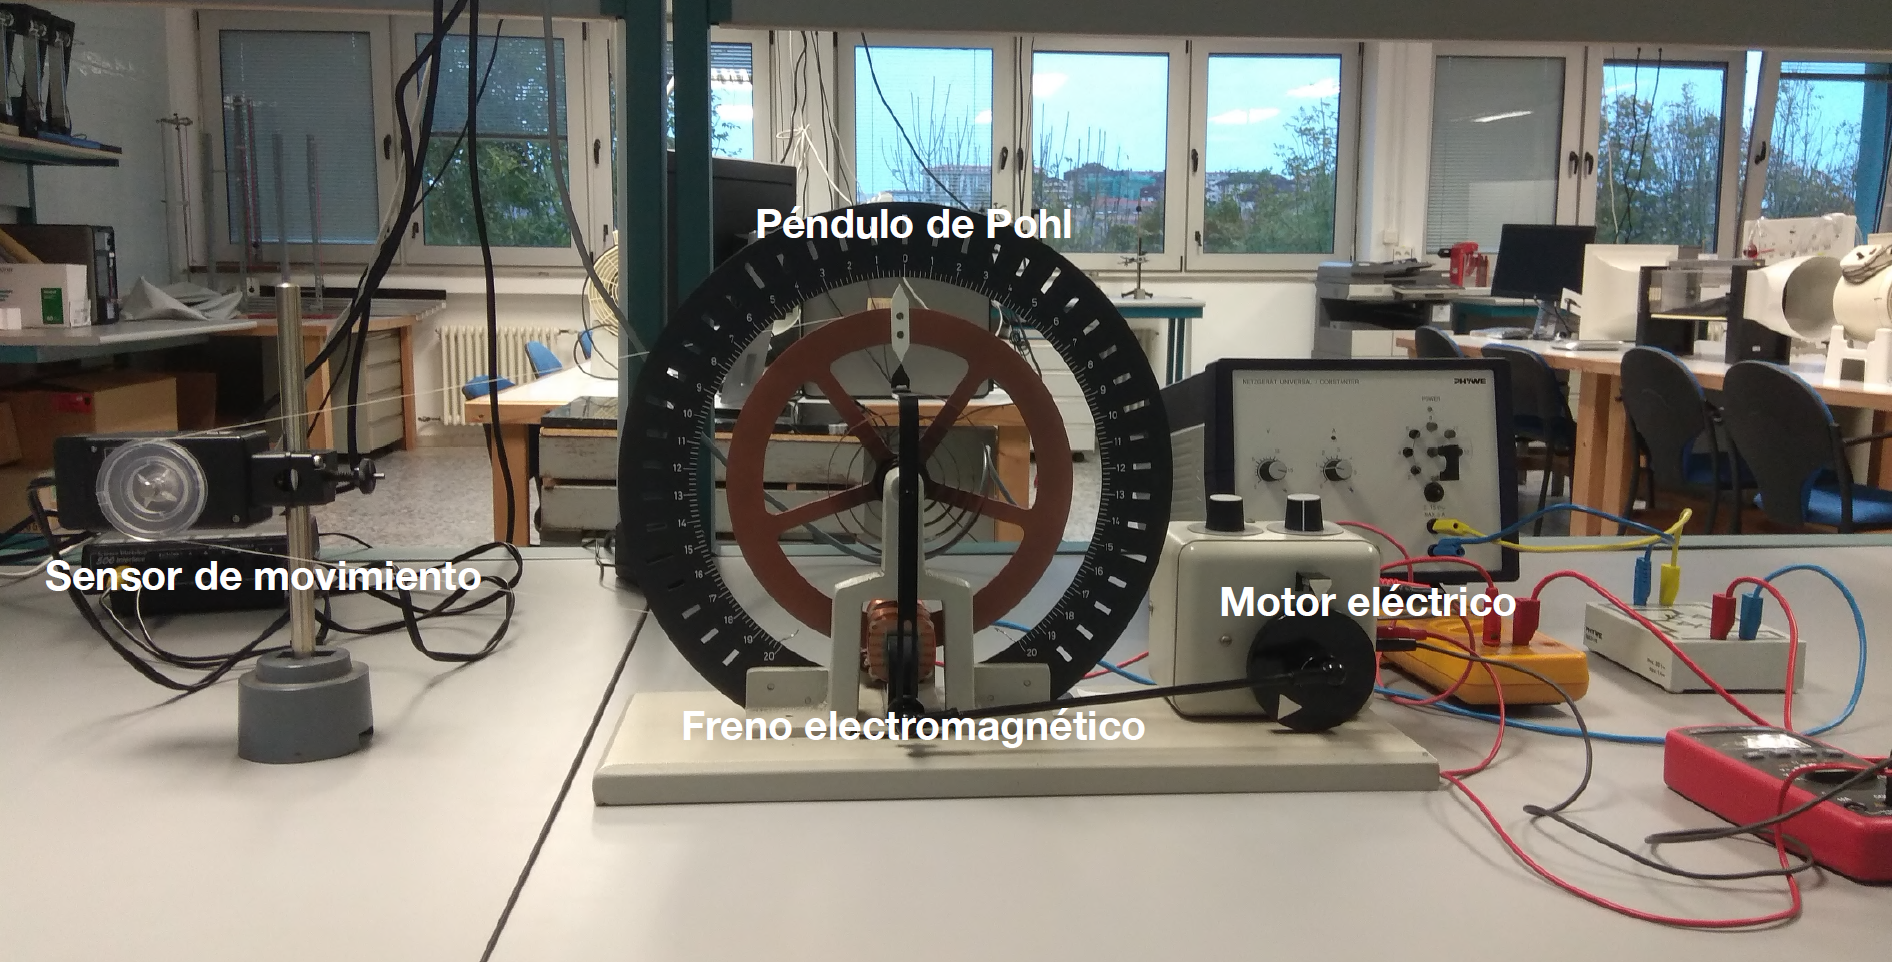
\includegraphics[width=1.0\textwidth]{figuras/pohl_Figura_1b.png}
\end{center}
\vspace*{-0.6cm}
\caption[]{\label{pohl}{P\'endulo de torsi\'on de Pohl. En la parte izquierda de la imagen se puede ver el sensor de movimiento, el cual est\'a conectado al p\'endulo por un hilo. En la base del p\'endulo se encuentra el freno electromagn\'etico y a su derecha est\'a el motor el\'ectrico causante de las oscilaciones forzadas.}}
\end{figure}


\section{Desarrollo}

Estima el factor de conversi\'on entre la medida del sensor de rotaci\'on y el \'angulo $\phi$.

\subsection{Oscilaciones libres}

Mide en primer lugar el per\'iodo $T$ de las oscilaciones libres sin conectar el freno electromagn\'etico, utilizando 5 oscilaciones para dos amplitudes iniciales diferentes: una menor $A_{12}$ de 12 muescas, y una mayor $A_{19}$ de 19 muescas. A partir del per\'iodo calcula la frecuencia $\omega = 2\pi/T$ con su error. Compara los resultados obtenidos para las dos amplitudes iniciales. {\bf Utiliza la mayor de las dos amplitudes iniciales para el resto de las medidas libres y amortiguadas.} Para obtener el valor del coeficiente de amortiguamiento $\gamma$ mide los m\'aximos (o m\'inimos) de la amplitud de las oscilaciones y los tiempos $t_n$ en los que se observan. Determina el valor del coeficiente de amortiguamiento $\gamma$ con su error mediante un ajuste lineal de los datos obtenidos. Analiza si el per\'iodo disminuye o aumenta de una oscilaci\'on a la siguiente.

\subsection{Oscilaciones amortiguadas}

Conecta el freno electromagn\'etico para el valor 6~V del potencial de la fuente de alimentaci\'on, y repite las medidas del per\'iodo $T$ y del coeficiente de amortiguamiento $\gamma$ para la amplitud inicial $A_{19}$. A partir del per\'iodo calcula la frecuencia $\omega$ con su error. Compara con el valor te\'orico $\omega_A = \sqrt{\omega_0^2 - \gamma^2}$. Utiliza para $\omega_0$ el valor obtenido para las oscilaciones con el freno desconectado. Analiza si el per\'iodo disminuye o aumenta de una oscilaci\'on a la siguiente. Compara el per\'iodo con el obtenido para el caso sin freno para oscilaciones con amplitudes similares.

\subsection{Oscilaciones forzadas}

Desconecta el freno. Conecta el motor a la fuente de alimentaci\'on. Observa cualitativamente la diferencia de fase $\delta$ entre las oscilaciones del disco (flecha blanca) y las del resorte unido al motor (flecha negra) para frecuencias de forzamiento $\Omega$ muy inferiores y muy superiores a $\omega_0$. Mide la amplitud $A$ y la frecuencia $\Omega$ de las oscilaciones forzadas estacionarias para diferentes valores de la frecuencia del motor. Anota los valores del voltaje. {\bf Para medir las amplitudes y frecuencias de las oscilaciones forzadas estacionarias se debe esperar hasta que desaparezcan los transitorios.} Las amplitudes de oscilaci\'on se deben medir como la media de las desviaciones del p\'endulo a izquierda y derecha, ya que posiblemente el punto intermedio de la oscilaci\'on no sea el cero de la escala. En las proximidades de la frecuencia de resonancia controla la variaci\'on de la frecuencia mediante el ajuste fino. Representa gr\'aficamente la amplitud de oscilaci\'on estacionaria $A$ frente a la frecuencia $\Omega$ (curva de resonancia). Estima el valor de la frecuencia de resonancia $\Omega_r$. Compara el resultado con la frecuencia obtenida para las oscilaciones libres y con el valor te\'orico dado por $\Omega_r = \sqrt{\omega_0^2 - 2\gamma^2}$. {\bf NOTA: parar con la mano para iniciar una medida para un voltaje nuevo, proporcionando unas condiciones iniciales reproducibles.}


\section*{Documenta en el cuaderno de laboratorio y en el informe}

Estimaci\'on del factor de conversi\'on entre la medida del sensor de rotaci\'on y el \'angulo $\phi$.

\subsection*{Oscilaciones libres}

\begin{itemize}

\item{Frecuencia con su error para dos amplitudes iniciales diferentes.}
\item{Coeficiente de amortiguamiento $\gamma$ con su error para la mayor amplitud inicial.}
\item{An\'alisis de la variaci\'on del per\'iodo de una oscilaci\'on a la siguiente.}

\end{itemize}

\subsection*{Oscilaciones amortiguadas}

\begin{itemize}

\item{Frecuencia y coeficiente de amortiguamiento con sus errores para la mayor amplitud.}
\item{Representa {\bf en la misma figura} los ajustes realizados para obtener los coeficientes de amortiguamiento de las oscilaciones libres y amortiguadas.}
\item{Comparaci\'on de la frecuencia obtenida con el valor te\'orico $\omega_A$.}
\item{An\'alisis de la variaci\'on del per\'iodo de una oscilaci\'on a la siguiente.}
\item{Comparaci\'on del per\'iodo con el caso sin freno para oscilaciones con amplitudes similares.}

\end{itemize}

\subsection*{Oscilaciones forzadas}

\begin{itemize}

\item{Curva de resonancia, es decir, amplitud estacionaria frente a la frecuencia.}
\item{Estimaci\'on de la frecuencia de resonancia $\Omega_r$. Comparaci\'on con la frecuencia obtenida para las oscilaciones libres y con el valor te\'orico.}

\end{itemize}


\section*{Apartado t\'ecnico}

El programa que usaremos para la realizaci\'on de esta pr\'actica es {\tt DataStudio}, el cual habr\'a que configurar siguiendo la Tabla~\ref{tabla:data-studio}.

\begin{table}[h!]
  \centering
  \begin{tabular}{l l l}
    \hline
    Opci\'on              & Crear experimento             & Create Experiment     \\
    Dispositivo           & Sensor de movimiento circular & Rotary Motion Sensor  \\
    Resoluci\'on          & Alta                          & High                  \\
    Escala lineal         & Polea grande (garganta)       & Large Pulley (Groove) \\
    Velocidad de muestreo & 200~Hz                        & 200~Hz                \\
    \hline
  \end{tabular}
  \caption{Par\'ametros de {\tt DataStudio}.}
  \label{tabla:data-studio}
\end{table}


%-------------------------------------------------------------------------------
% Bibliografia
%-------------------------------------------------------------------------------

\begin{thebibliography}{X}

\bibitem{tipler}
  P.~A.~Tipler y G.~Mosca,
  \textit{F\'isica para la ciencia y la tecnolog\'ia}.\\
  Editorial Revert\'e, 2005, $5^{a}$ edici\'on, Volumen 1, Cap\'itulo 13.

\bibitem{ablanque}
  J.~Anderson, J.~C.~Losada, A.~S.~Sanz, F.~J.~Arranz y R.~M.~Benito,
  \textit{Laboratorio asistido por ordenador: oscilaciones regulares y ca\'oticas en el p\'endulo de Pohl}.\\
  Revista Espa\~nola de F\'isica, {\bf 20} (4), pp. 34-39, 2006.

\bibitem{morin}
  D.~Morin,
  \textit{Introduction to Classical Mechanics: With Problems and Solutions}.\\
  Cambridge University Press, 2008.

\end{thebibliography}


%-------------------------------------------------------------------------------
% Fin del documento
%-------------------------------------------------------------------------------

\end{document}
